\section{Basics}
\subsection{Network composition}
A network consists of three elements:
\begin{itemize}
	\item \textbf{End systems}: can vary in size and usage
	\item \textbf{Intermediate systems}: these (e.g. routers) are the components that allow the network to work.
	\item \textbf{Links}: they connect the end systems and can be \textit{optical}, \textit{copper} or \textit{wireless}. Even if wireless is becoming more and more important, cables are still fundamental (undersea cables, underground cables).
\end{itemize}

\begin{question}[Why fiber optic?]
	Because this medium has not reached it's maximum and still has a huge potential of \textbf{bandwidth}. Also, while copper cable start acting as an \textbf{antenna} (and a receiver), disturbing near copper cable, fiber optic doesn't have this problem. Furthermore, copper cables need amplifiers which increase \textbf{latency}.
\end{question}

\begin{question}[Why copper?]
	It's \textbf{cheaper} and \textbf{easier} to handle.
\end{question}

\begin{question}[Why cables over wireless?]
	Because of \textbf{stability} and \textbf{latency}. Usually the problem is tampered by buffers but obviously it doesn't work with interactive applications.
\end{question}

\begin{question}[What are threats to cable?]
	
\end{question}

\subsection{Communication principles}
There are two basics principles:
\begin{itemize}
	\item \textbf{Synchronous}: joint action of sender and receiver. Requires \textbf{waiting} until all parties are ready (e.g. phone calls)
	\item \textbf{Asynchronous}: sender and receiver operate decoupled (e.g. SMS, email). Requires \textbf{buffering}.
\end{itemize}

\begin{note}
	There is also \textbf{isochronous}, which means the messages are sent every predetermined amount of time.
\end{note}

\subsubsection{Direction}
Communication channels may allow traffic flow in different directions:
\begin{itemize}
	\item \textbf{Simple duplex}: one direction
	\item \textbf{Half-duplex}: both directions in different moments
	\item \textbf{Full-duplex}: both directions at the same time
\end{itemize}
\subsubsection{Distribution}
The communication distribution can happen in different ways:
\begin{itemize}
	\item \textbf{Unicast}: one to one
	\item \textbf{Broadcast}: one to all
	\item \textbf{Multicast}: one to a subset
	\item \textbf{Anycast}: one to the nearest, e.g. when requesting to a redundant database you don't care which one responds
	\item \textbf{Concast}: many to one, e.g. we collect sensor data and send it to one
	\item \textbf{Geocast}: one to a certain region
\end{itemize}
\begin{note}
	Even if multicast would be easier and cheaper, companies usually go for unicast because they want to know who the clients are.
\end{note}

\begin{note}
	Broadcast guarantees anonymity while multicast does not.
\end{note}

\subsubsection{Topologies}
The main topologies are:
\begin{itemize}
	\item \textbf{Full mesh}: too expensive
	\item \textbf{Chain}: in cars and trains
	\item \textbf{Star}: ideal for switches
	\item \textbf{Partial mesh}: the best compromise
	\item \textbf{Tree}: not ideal for big networks since if you cut a side, you lose contact
\end{itemize}

\subsection{Sharing}
\subsubsection{Cons}
Sharing may create a lot of problems, like \textbf{bottlenecks}: links and intermediate nodes are shared between end systems. One solution may be to \textit{reroute} or to start \textit{dropping packets} (e.g. when streaming the resolution lowers down).
\subsubsection{Pros}
At the same time, sharing means more efficient (less expensive) mechanism to \textbf{exchange data} between different components of distributed systems and \textbf{minimize blocking} due to multiplexing.

\subsubsection{How?}
There are two possible ways of sharing:
\begin{itemize}
	\item \textbf{Reservation}: you reserve in advance the resource so that it is guaranteed, e.g. remote surgery. When the peak demand and the flow duration varies, there are two options:
	\begin{enumerate}
		\item \textit{First Come First Served}
		\item Everyone gets $10Mbps$
	\end{enumerate}
	It is implemented with \textbf{circuit-switching}: establishes dynamically a dedicated communication channel. It has predictable performance and a simple and fast switching but it's inefficient for bursty traffic, complex to setup and not easily adaptive to failures.
	
	\item \textbf{On-demand}: when there is a resource available you take it (variable \textit{delay}, \textbf{jitter}), e.g. email. It is implemented with \textbf{packet-switching}: splitting the resource in packets and multiplex them. Much more flexible but requires buffers, packets overhead and has unpredictable performances.
\end{itemize}

\begin{observation}
	It all depends on the application. Each flow has a \textbf{peak rate} and an \textbf{average rate}.To decide if \textit{reservation} works well for a specific case, we must look at the ratio $\frac{P}{A}$. If it's small then it works well, otherwise it's wasting resources.
\end{observation}

\subsection{Internet}
Internet is a network of networks. It enables processes on different hosts to exchange data: it's a bit delivery system.\\
ISPs enable you to access and use Internet services: well defined and commonly required functions. There are two roles: \textbf{client} and \textbf{server} that can be on different machine (or not, like with P2P).

\begin{definition}[Internet]
	The set of all reachable parties (IP addresses).
\end{definition}

\subsection{Protocols, layer and standards}
\begin{definition}[Digital Data Communication]
	\textit{Processing} and \textit{transport} of digital data between interconnected computers.
\end{definition}

\begin{definition}[Data]
	\textbf{Representation} of facts, concepts and statement in a formal way which is suitable for communication, interpretation and processing by human beings or technical means.
\end{definition}

\begin{note}
	\textbf{Information} is different from the data.
\end{note}

\begin{definition}[Signal]
	A signal is the physical representation of data by spatial or timely variation of physical characteristics.
\end{definition}

In this context we need rules of communication for the different devices to communicate: we have heterogeneous computer architectures, network infrastructure  and distributed application. A \textbf{protocol} is a conversational convention, consisting of syntax and semantic.

\begin{definition}[Protocol]
	Protocols define format, order of messages sent and received among network entities, and actions taken on message transmission and receipt.\\
	A protocol is a set of \textbf{unambiguous} specifications defining how processes communicate with one another through a connection (wire, radio etc.).
\end{definition}

\noindent To provide structure to the design of networks protocols, network designers organize protocols in \textbf{layers}. We use two models, either the ISO/OSI or the TCP/IP.
\begin{center}
	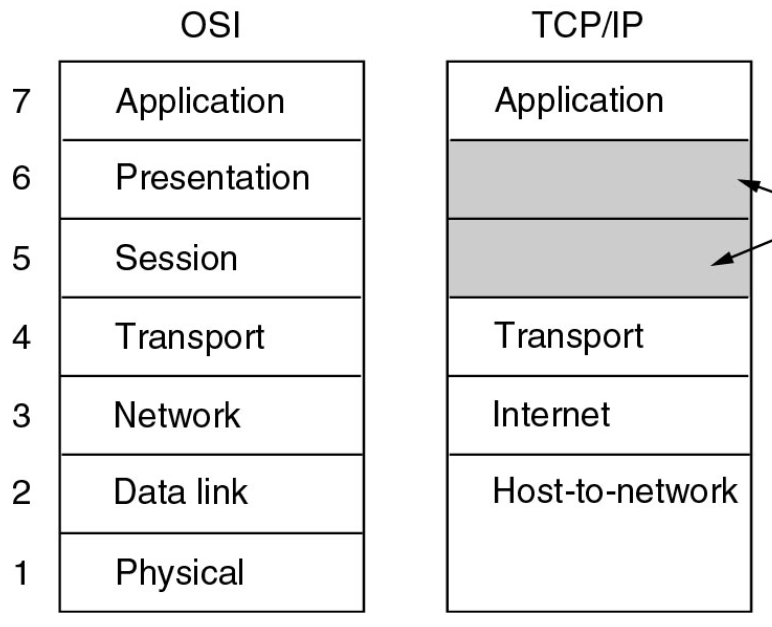
\includegraphics[scale=0.3]{isoosi.png}
	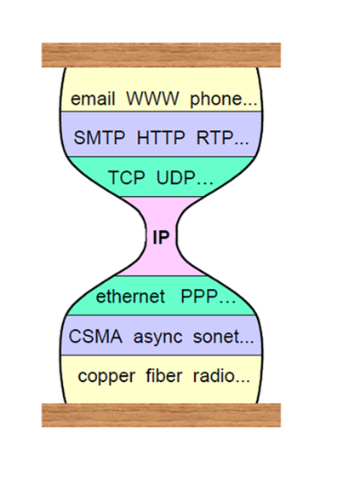
\includegraphics[scale=0.4]{hourglass.png}
\end{center}

\noindent All the different layers need additional information, which is added via \textbf{headers} to the data payload via \textbf{encapsulation}. This could cause a lot of \textbf{overhead}.\\
All the protocols rely on the Internet Protocol. This maximizes \textbf{interoperability} and does not ensure anything, therefore no one has expectations.

\subsection{Quality of service}
To define the quality of communication we check:
\begin{itemize}
	\item \textbf{Technical performance}: delay, jitter, throughput, data rate, etc.
	\item \textbf{Costs}
	\item \textbf{Reliability}: fault tolerance, system stability, immunity, availability
	\item \textbf{Security and Protection}: eavesdropping, authentication, denial of service, etc.
\end{itemize}

\subsubsection{Latency}
The main parameters we check are:
\begin{itemize}
	\item \textbf{One-way delay}: measured in seconds
	\begin{equation}
		d_1 = t'_1-t_1
	\end{equation}
	\item \textbf{Round-trip-time}: measured in seconds
	\begin{equation}
		r_1 = t_2 - t_1
	\end{equation}
	It should also integrate the processing time of the other device.
\end{itemize}

\subsubsection{Stability}
The main parameter that measures stability is the \textbf{Jitter}. It's measured in seconds and calculated using the delay:
\begin{equation}
	d_i = t'_i - t_i \quad\quad j_i = d_{i+1} - d_i
\end{equation}

\subsubsection{Capacity}
From a capacity perspective, we measure the \textbf{throughput} in $\frac{bit}{s}$ as follows:
\begin{equation}
	T=\frac{\sum \text{data}_i}{\Delta t}
\end{equation}
The \textbf{goodput} instead, is the amount of \textbf{useful} throughput from a user perspective.

\begin{note}
	\textbf{Bandwidth} is used for the description of the channel characteristics.
\end{note}

There is also the \textbf{Delay-Throughput-Produc} which measures how much data can be on the medium itself while traveling. E.g. with a connection of $1Mbps$ that has $200 ms$ of delay we have 
\begin{equation*}
	1 Mbps \times 0.2s = 200kbit
\end{equation*}